\documentclass[a4paper,norsk, 10pt]{article}
\usepackage[utf8]{inputenc}
\usepackage{verbatim}
\usepackage{listings}
\usepackage{graphicx}
\usepackage[norsk]{babel}
\usepackage{a4wide}
\usepackage{color}
\usepackage{amsmath}
\usepackage{float}
\usepackage{amssymb}
\usepackage[dvips]{epsfig}
\usepackage[toc,page]{appendix}
\usepackage[T1]{fontenc}
\usepackage{cite} % [2,3,4] --> [2--4]
\usepackage{shadow}
\usepackage{hyperref}
\usepackage{titling}
\usepackage{marvosym }
%\usepackage{subcaption}
\usepackage{subfig}
\usepackage[noabbrev]{cleveref}
\usepackage{cite}
\usepackage{todonotes}


\setlength{\droptitle}{-10em}   % This is your set screw

\setcounter{tocdepth}{2}

\lstset{language=c++}
\lstset{alsolanguage=[90]Fortran}
\lstset{alsolanguage=Python}
\lstset{basicstyle=\small}
\lstset{backgroundcolor=\color{white}}
\lstset{frame=single}
\lstset{stringstyle=\ttfamily}
\lstset{keywordstyle=\color{red}\bfseries}
\lstset{commentstyle=\itshape\color{blue}}
\lstset{showspaces=false}
\lstset{showstringspaces=false}
\lstset{showtabs=false}
\lstset{breaklines}
\title{AST5220 Milestone4}
\author{Daniel Heinesen, daniehei}
\begin{document}
\maketitle
\section{Introduction}
So far we have found out how the Universe expands, found the number density of free electrons and how this impact the mean free path of the photons. We have then used this to calculate how initial perturbations after inflation would have evolved through till today. We are now ready to use all of this to find what we are after: The power spectrum of the Cosmic Microwave Background (CMB). 

\todo{Maybe summarize the method and theory?}

\section{Theory}
We are after the power spectrum

\begin{equation}
C_l = \langle |a_{l,m}|^2\rangle = \int \frac{d^3 k}{(2\pi)^3}|a_{l,m}|^2.
\end{equation}
We need to integrate since since we have Fourier transformed all out quantities. $a_{l,m}$ comes from the fact that we observe the temperature of the CMB projected on a sphere, meaning that we can write it as 
\begin{equation}
T(\hat{n}) = \sum a_{l,m} Y_{l,m}(\hat{n}),
\end{equation}
where $Y_{l,m}$ are spherical harmonics and $a_{l,m}$ the coefficients containing the actual physics of the temperature field. Instead of finding $|a_{l,m}|^2$ directly, we can instead define $|a_{l,m}|^2 = P(k)\Theta_l^2$, where $P(k)$ is the primordial power spectrum and $\Theta_l$ is the so called \textit{transfer function} which contain all the information about how the power spectrum has evolved from inflation and until today. We can get the primordial power spectrum from the Harrison Zel'dovich spectrum 
\begin{equation}
\frac{k^3}{2\pi^2}P(k) = \left(\frac{ck}{H_0}\right)^{n_s - 1},
\end{equation}
where $n_s$ is the spectral index. We can now write the power spectrum as
\begin{equation}\label{eq:Cl}
C_l = \int^{\infty}_{0}\left(\frac{ck}{H_0}\right)^{n_s - 1} \Theta_l^2(k) \frac{dk}{k}.
\end{equation}
We now need to find the transfer function $\Theta_l$. As the choice of name implies, this is perturbation of the $l^{th}$ momentum we found in milestone 3. The problem is the while we calculated these up to $l = 6$ the CMB spectrum is given for $l>1200$. Calculating all these perturbations with the use of the method in milestone 3 is slow, so we need a faster way. Thanks to Zaldarriaga and Seljak we can calculate the momenta in minutes and not hours. They found the so called \textit{line of sight integration} method. This means that instead of doing a multipole expansion of the temperature, then solve the differential equations, we instead solve the equations and then expand. This means that we can write, after some calculation,

\begin{equation}\label{eq:Theta}
\Theta_l(k,x=0) = \int_{-\infty}^{0} \tilde{S}(k,x)j_l(k(\eta_0 - \eta)) dx,
\end{equation}
where $j_l(k(\eta_0 - \eta))$ is the $l^{th}$ spherical Bessel function evaluated at $k(\eta_0 - \eta)$, and $\tilde{S}$ the source function. The source function is defined as

\begin{equation}\label{eq:S}
\tilde{S}(k,x) = \tilde{g}\left(\Theta_0 + \Psi + \frac{1}{4}\Pi\right) +e^{-\tau}\left(\Psi' - \Phi'\right)  - \frac{1}{ck}\frac{d}{dx}\left(\mathcal{H}\tilde{g}v_b\right) + \frac{3}{4c^2k^2}\frac{d}{dx}\left[\mathcal{H}\frac{d}{dx}\left(\mathcal{H}\tilde{g}\Pi\right) \right],
\end{equation}
where (here) $\Pi = \Theta_2$. The source function can be thought of a function describing all the different things a photon encounters on our way to us that decreases or increases its energy. The first term describes the Sachs-Wolfe effect -- the loss of energy as a function climbs out of a gravitational potential --, the second term describes the integrated Sachs-Wolfe effect -- if the gravitational potential have change from when a photon enters to it leaves, this affects its energy --, and the third term is the Doppler term. Notice that the source function only needs temperature momenta up to $\Theta_2$, so we do not need to solve the differential equations for $l$ higher than $2$. In reality, since we use an approximation to find $\Theta_{lmax}'$, there is a small error in the highest momentum. If we solve for $l$ up to $6$ this error is small enough for $\Theta_2$ and below, that the error can be ignored.

\todo{Maybe write down all the equations used to calc S}

\section{Method}
The method consists of two parts: Calculating the source function and integrating everything to get the final power spectrum.

\subsection{Source Function}
We want the source function from the start of recombination until today. From milestone 3 we have all the quantities we need to calculate $\tilde{S}$, but not with the precision we want. So with our quadratic $k$ grid with $100$ $k$s and our $x$ grid with $500$ points, we can find an initial grid of $\tilde{S}(k,x)$. We can then spline this 2D array. With new, finer $k$ and $x$ grids, both with $5000$ points in the same intervals, we can use the spline to get a new $\tilde{S}$ array with a finer grid. It is these grid we are going to use for the rest of the calculations.

Both $\tilde{S}$ and $j_l$ are saved in binary files, so that if all the calculations below needs to be run multiple times -- for any reason --, we don't need to solve all the differential equations and calculate the Bessel functions again.

\subsection{Integrating Everything}
To find $\Theta_l$ we see from eq. \eqref{eq:Theta} that we need to find the spherical Bessel functions. Fortunately we are given functions to find these. But we need to save the Bessel function in a grid for each $l$ and for $5400$ values from $0$ to $3500$. For each $l$ we will spline the Bessel function for use later.

We can now use eq. \eqref{eq:Theta} to find the transfer functions $\Theta_l$. This integration was done with a simple trapezoidal integration \todo{Check is this was used, and update if something else is used!}. 

We then integrate the $\Theta_l$s with the primordial power spectrum to get the $C_l$s, eq. \eqref{eq:Cl}. This again is done via an Euler Scheme \todo{Change is something else is used!}. We start by finding $C_l$ for $44$ $l$s from $1$ to $1200$. We then spline and retrieve a $C_l$ for each $l$ in the same interval. We then normalize as $C_l\cdot l(l+1)/2\pi$, and we have our long sought after power spectrum. 

All the calculation are in the first instance done with a default set of parameters $\Omega_b$, $\Omega_m$, $\Omega_r$, $n_s$ and $h$. With these parameters, the resulting power spectrum are not a good fit for the one observed by the Planck Satellite, so we need to find the correct values for the parameters. This is done by adjusting the parameters one by one and seeing who this affect the power spectrum, this making it possible to infer how we can change the parameters to fit the observed power spectrum.

\todo{Maybe write more?}

\section{Results}

The first plots we are going to look at source function and the transfer function. 

\todo[inline]{Change font of axis!!!}

\begin{figure}
\centering
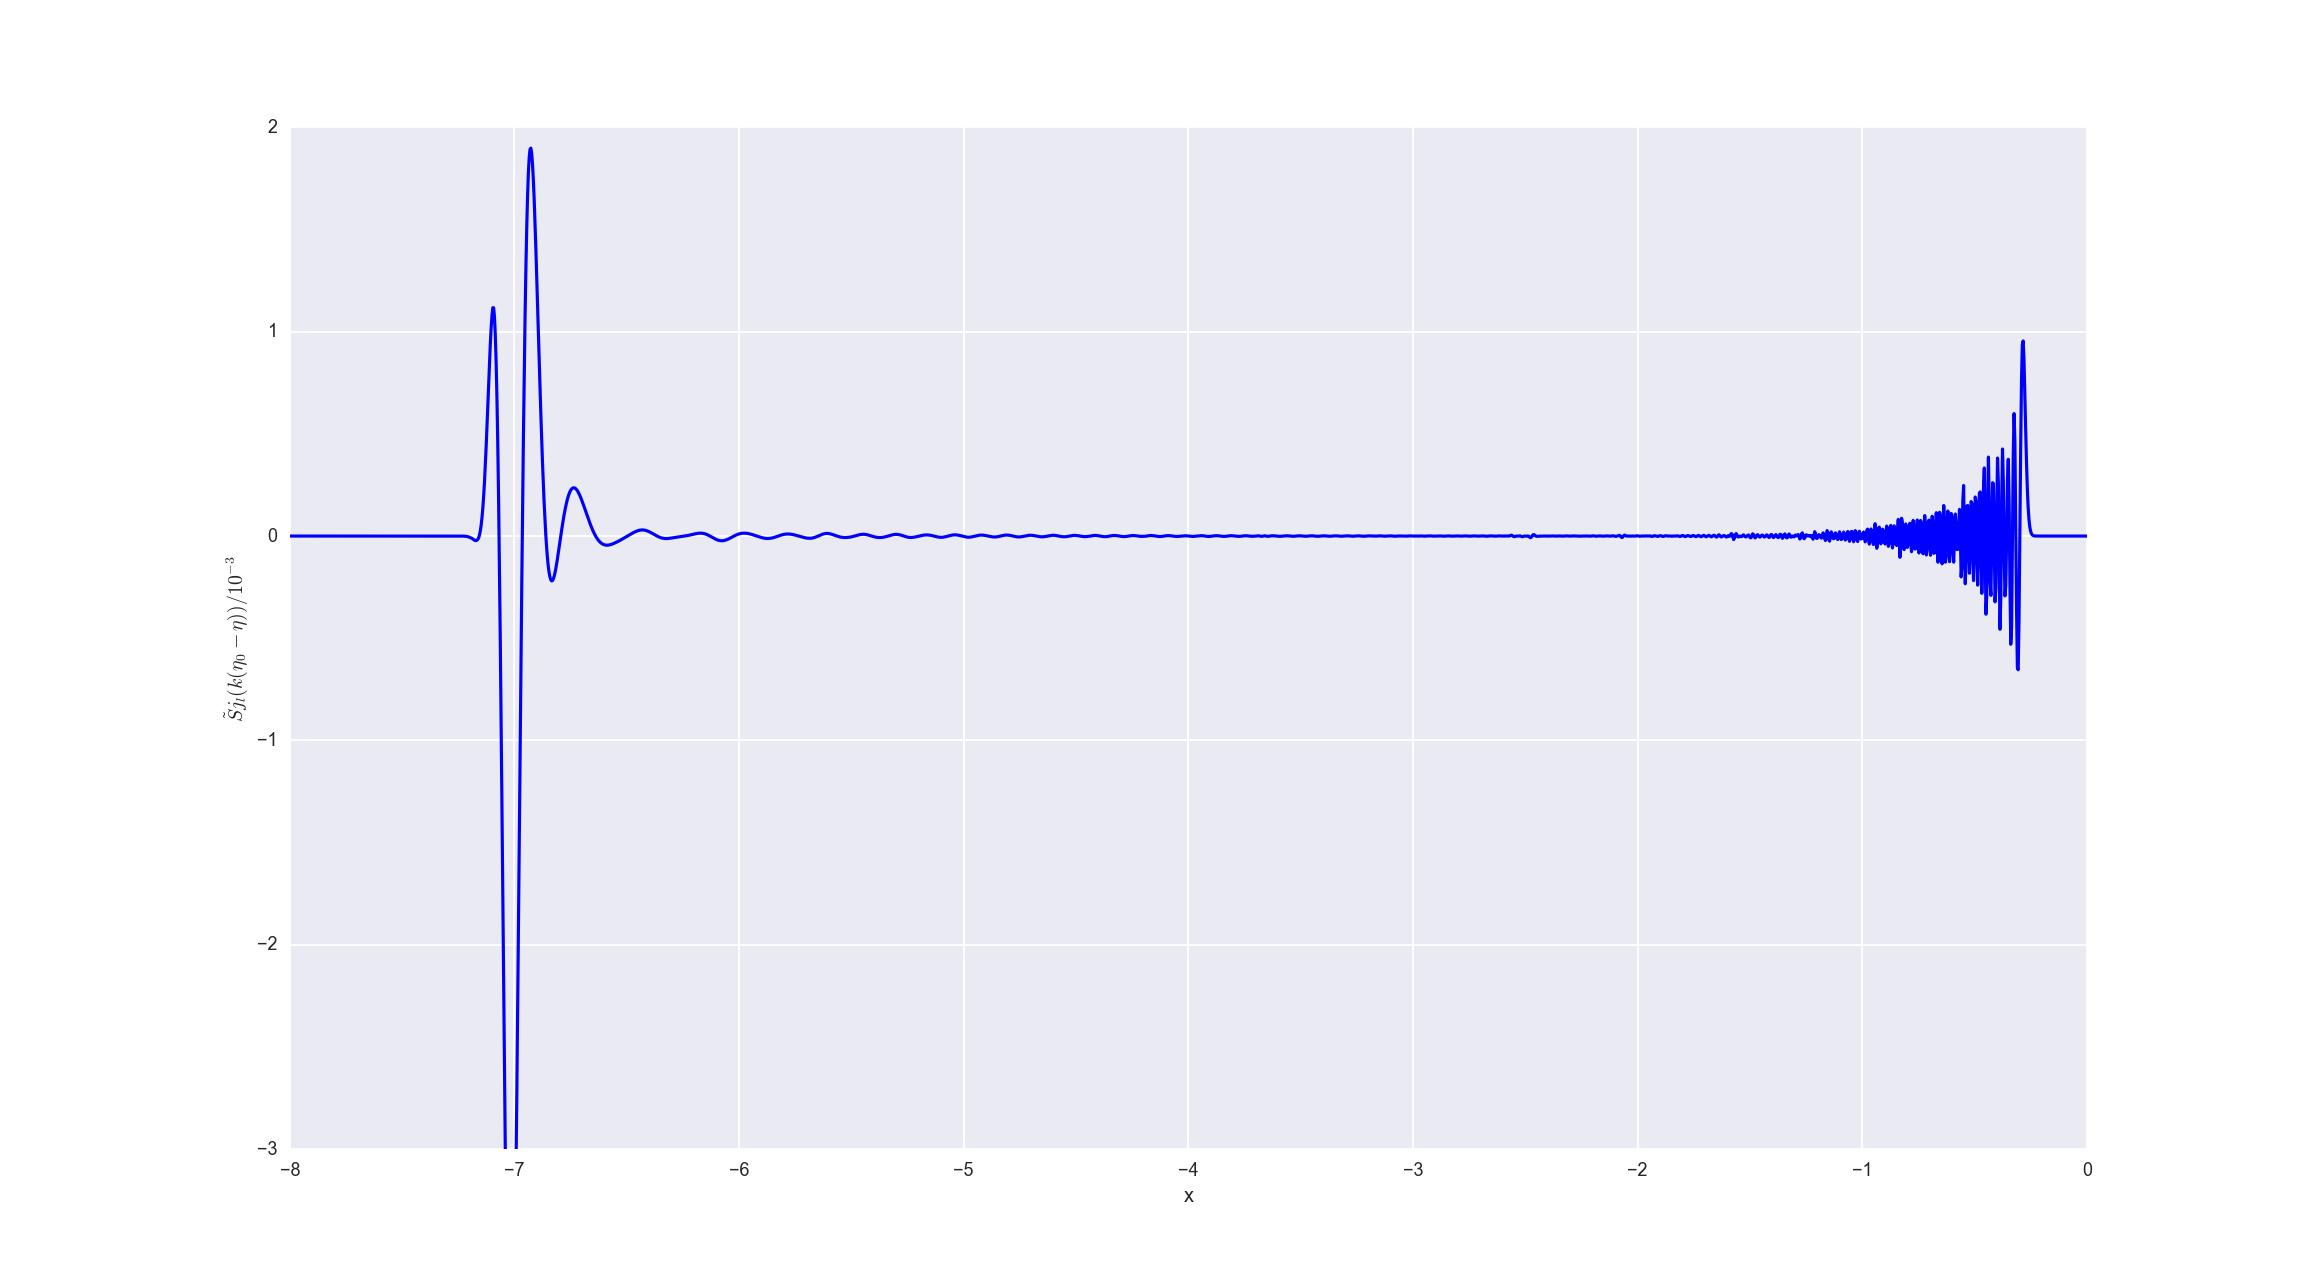
\includegraphics[scale=0.25]{sjl.png}
\caption{This shows the source function multiplied with the spherical Bessel function for $l=100$ and $k = 340\cdot H_0/c$.}\label{fig:sjl}
\end{figure}

\begin{figure*}[!htbp]
\centering
\begin{tabular}{@{}ccc@{}}
\subfloat[The gravitational curvature potential $\Phi$. As with the matter, perturbations before entering the horizon are constant. The three larges $k$s (corresponding to smalles scales) will enter the horizon during radiation domination, rapidly decay before starting to oscillate. The oscillation will be dampend, and (after the start of matter domination) the potential will become constant. The largest scales will enter after radiation-matter equvalence, during which they will fall a bit and stay constant. Near present age, dark energy starts to dominate, and $\Phi$ starts to decrease.\label{fig:Phi}]{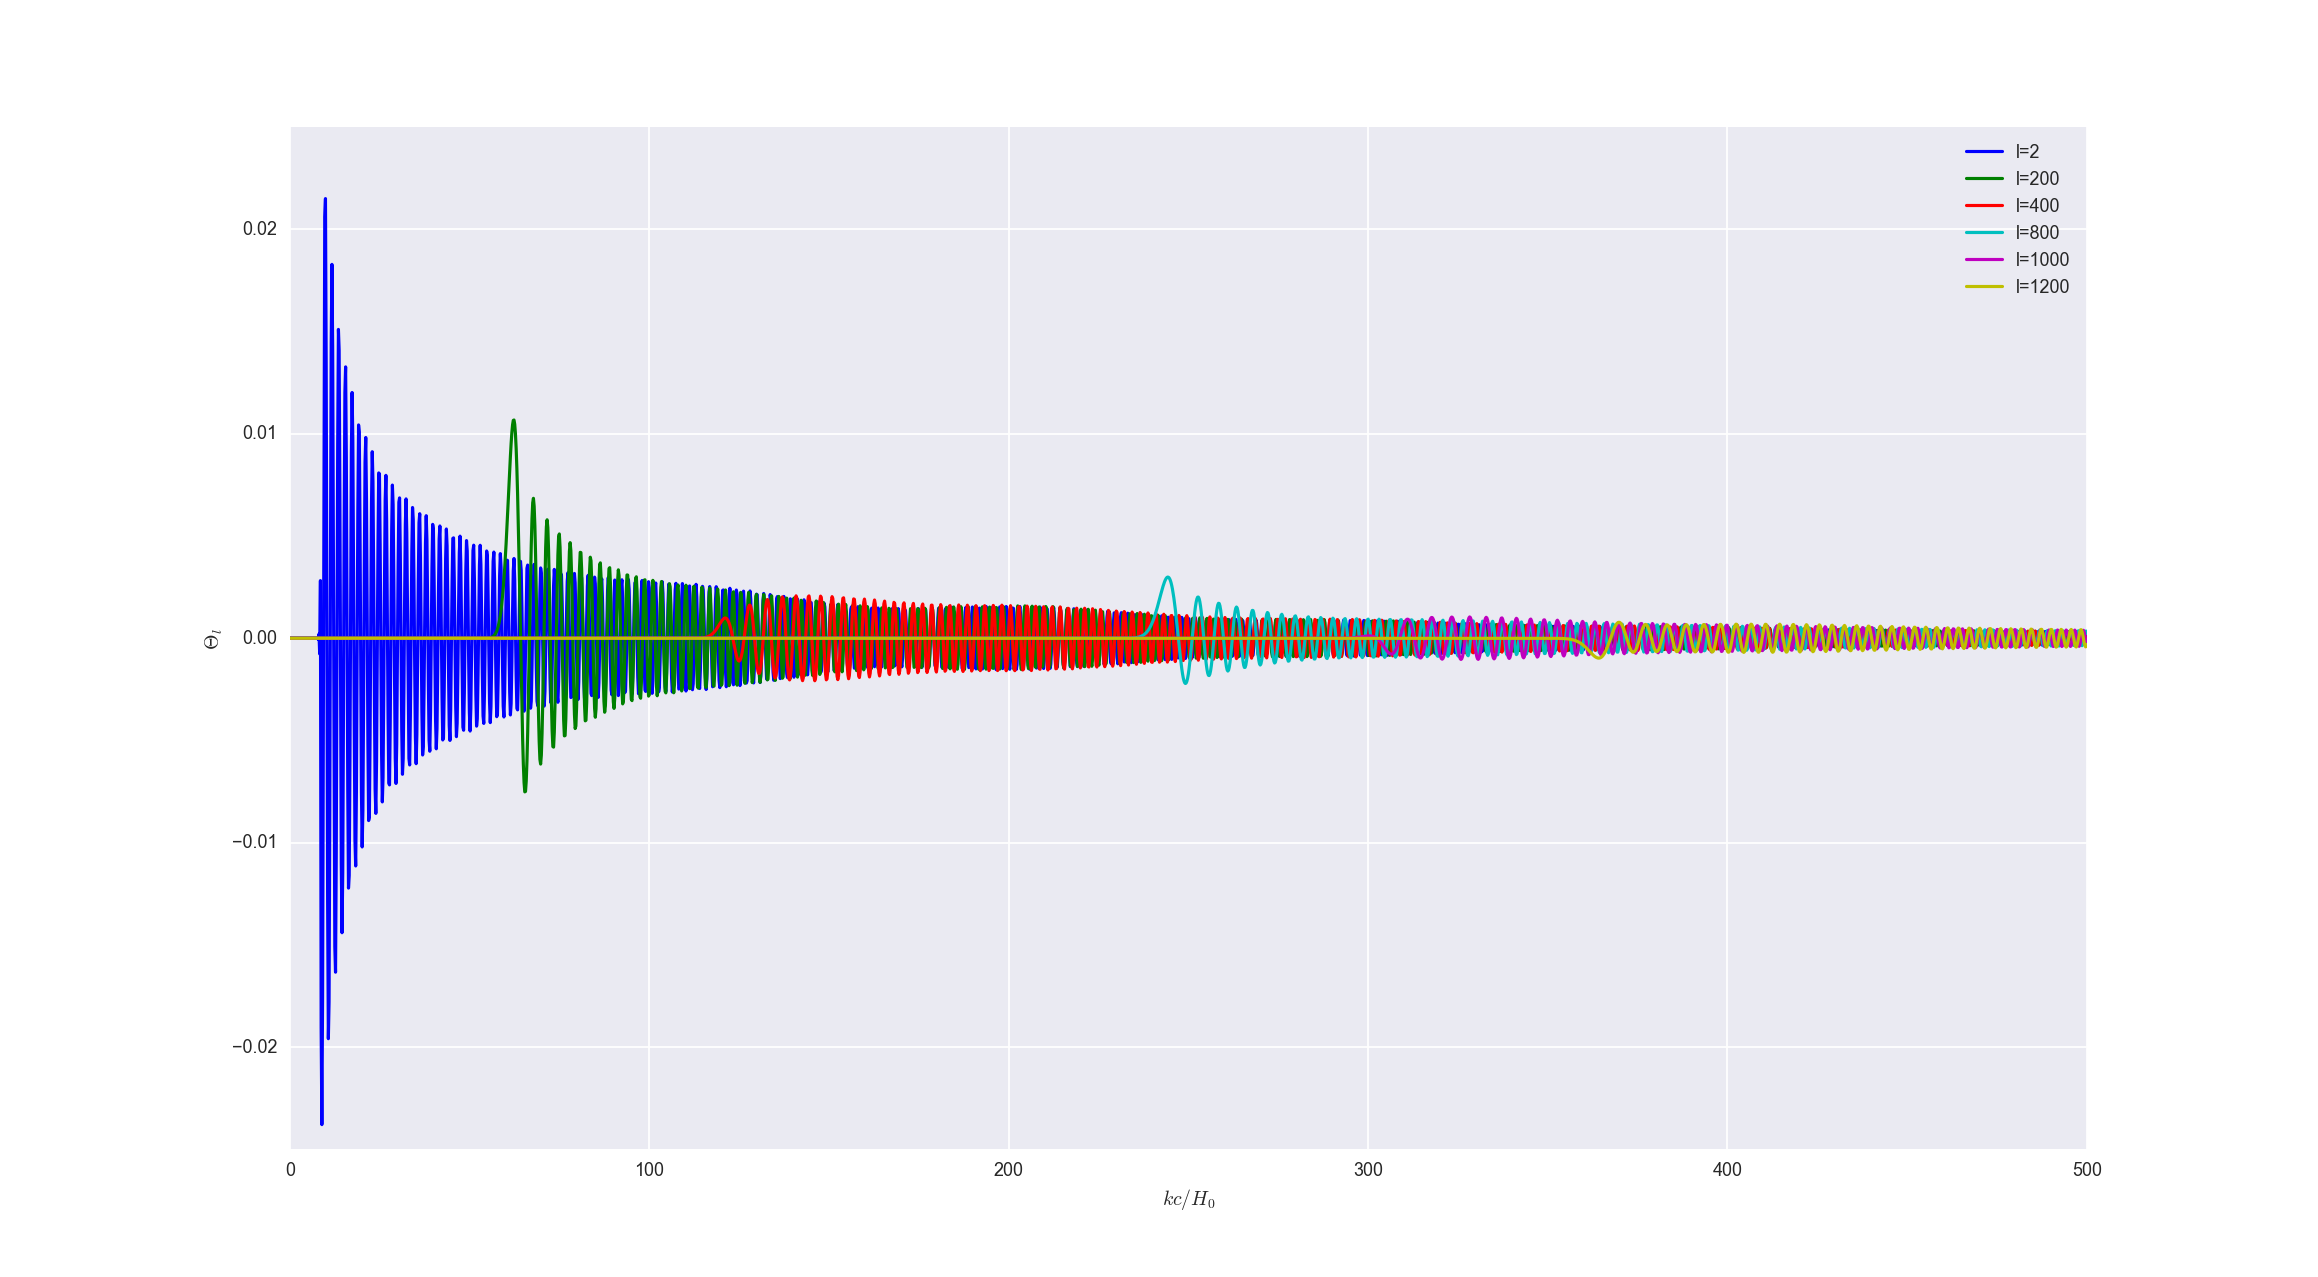
\includegraphics[width=0.5\textwidth]{theta_l.png}} & 
\subfloat[The Newtonian potential $\Psi$. This growth more or less the same as $\Phi$ decreses. We can approximate that $\Psi = - \Phi$.\label{fig:Psi}]{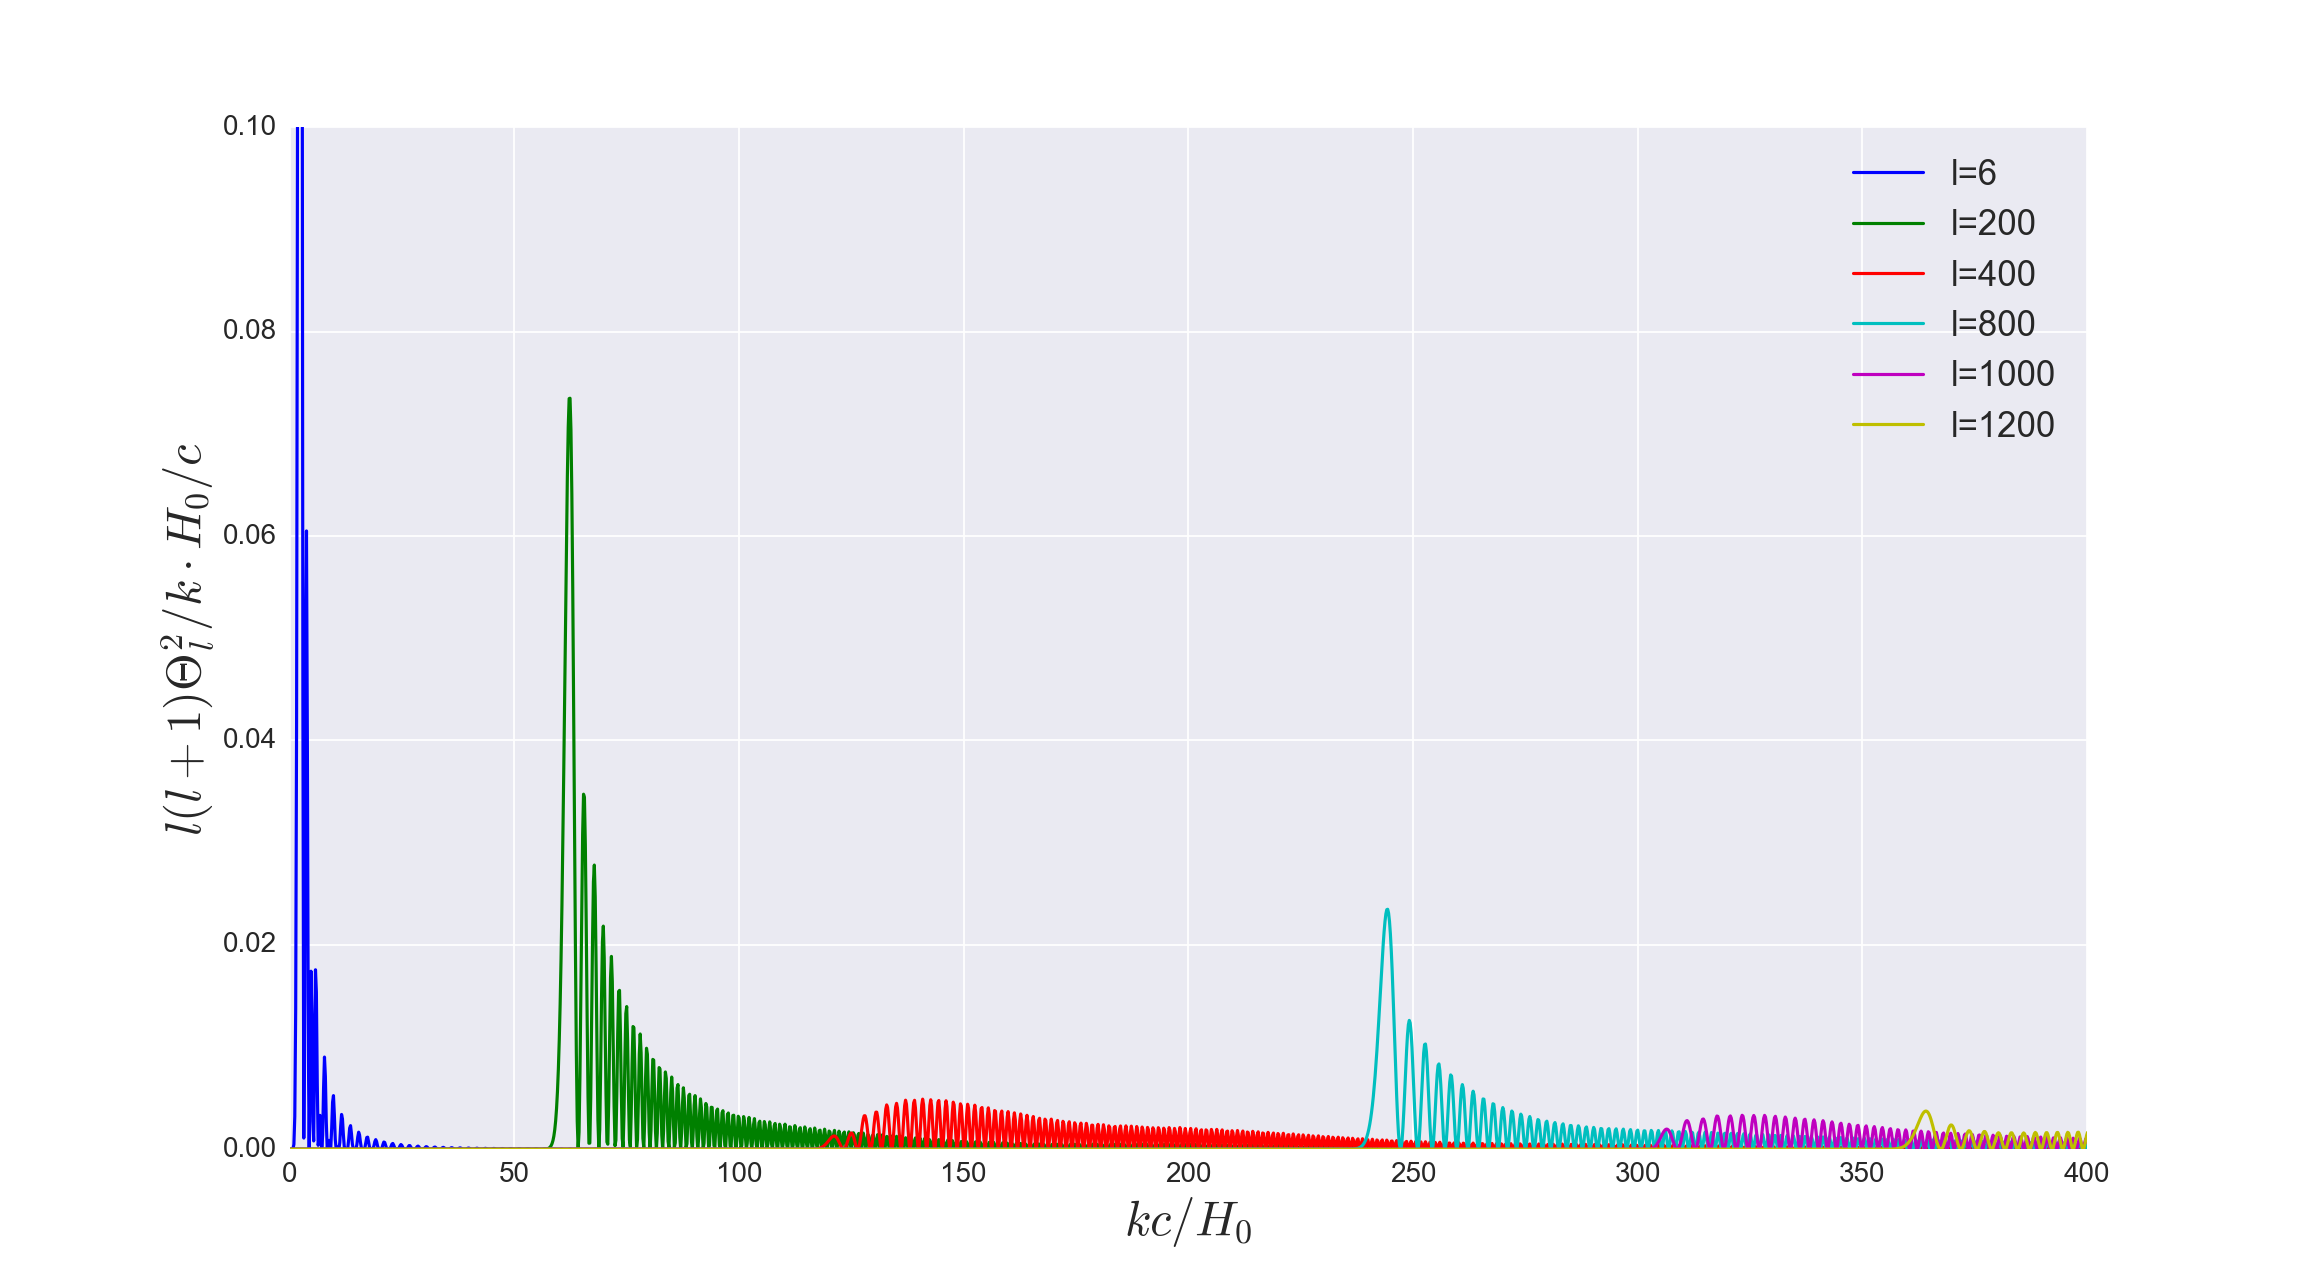
\includegraphics[width=0.5\textwidth]{theta_sq_k.png}} 
\end{tabular}
\caption[]{Plots showing the transfer function $\Theta_l(k)$ for a selection of $l$s.}
\label{fig:psi_phi}
\end{figure*}






\begin{thebibliography}{9}

\bibitem{callin}
  Callin, Peter,
  \textit{How to calculate the CMB spectrum},
  astro-ph/0606683
  2006.

\end{thebibliography}


\end{document}

